\documentclass[11pt]{article}

\usepackage[margin=1in]{geometry}
\usepackage{amsmath}
\usepackage{amssymb}
\usepackage{url}
\usepackage{booktabs}
\usepackage{graphicx}
\usepackage{longtable}
\usepackage{array}
\usepackage[colorlinks,bookmarksopen,bookmarksnumbered,citecolor=blue,urlcolor=blue,linkcolor=blue]{hyperref}
\usepackage{caption}

% S-prefixed table/figure numbering, per supplementary-material convention
\renewcommand{\thetable}{S\arabic{table}}
\renewcommand{\thefigure}{S\arabic{figure}}
\renewcommand{\thesection}{S\arabic{section}}

\title{Supplementary Information\\[4pt]
\large Sampling Design for Spatial Cluster Randomized Trials Under Heterogeneous Incidence}
\author{Andrew Walther, Ross Joseph Simpson, Jr., Ashkan Habib, and Feng-Chang Lin}
\date{}

\begin{document}
\maketitle

This document provides the reproducibility, parameter-grid, metric-formula, and
complete eight-design comparison material referred to in the main text as
``online supplementary material.'' All numeric values below were verified
directly against the simulation output files
\path{results/six_design_manuscript/six_design_summary.txt},
\path{results/six_design_manuscript/dissertation_results_extract.txt}, and
\path{results/eight_design_supplementary/eight_design_summary.txt}
(the last generated fresh for this document by
\path{code/14_manuscript_supplement_figures.R}). No number below is asserted
without a corresponding entry in one of these files.

Unless otherwise noted, all sections other than Section~\ref{sec:s6} present the
\textbf{six treatment assignment designs retained in the main text} (Checkerboard,
High Incidence Focus, Isolation Buffer, 2$\times$2 Blocking, Balanced Quartiles,
and Incidence-Guided Saturation Quadrants), ordered from best (lowest mean squared
error, MSE) to worst wherever a ranking is shown. Section~\ref{sec:s6} is the sole
section presenting all eight designs evaluated in the underlying simulation study,
including the two variants (Saturation Quadrants, Balanced Halves) dropped from the
main comparison as statistically redundant with a retained design.

\section{Reproducibility and Code Availability}
\label{sec:s1}

All simulation, estimation, and figure-generation code is organized as a
numbered pipeline in \texttt{code/}, sourced in dependency order:

\begin{center}
\small
\begin{tabular}{p{4.3cm}p{9.2cm}}
\toprule
Script & Role \\
\midrule
\path{01_spatial_setup.R} & $10\times10$ grid construction; rook/queen spatial weight matrices \\
\path{02_incidence_generation.R} & Baseline incidence generation (iid, spatial, Poisson modes) \\
\path{03_designs.R} & The eight treatment assignment designs (Section~\ref{sec:s5}) \\
\path{04_estimation.R} & DIM and MLE (\texttt{lagsarlm}) estimation of $\tau$, with CI extraction \\
\path{05_run_simulation.R} & Main orchestrator: parameter grid, seeding, simulation loop \\
\path{06_visualizations.R} & Plotting and tabulation functions \\
\path{10_statistical_comparisons.R} & Friedman/Nemenyi/Wilcoxon hypothesis testing \\
\path{12_six_design_statistical_comparisons.R} & Six-design re-analysis (statistical redundancy check) \\
\path{14_manuscript_supplement_figures.R} & Figures and tables for this document \\
\bottomrule
\end{tabular}
\end{center}

\subsection*{Seeding protocol}

Every simulated scenario uses a distinct, deterministic seed rather than a single
global seed for the whole run, so that any individual scenario can be reproduced
in isolation and re-ordering scenarios does not change their results. The seed for
scenario $(\text{inc\_mode}, \rho_X, \text{nb\_type}, \rho, \gamma,
\text{spill\_type}, \text{design\_id}, \tau)$ is

\begin{quote}
\texttt{scenario\_seed <- digest::digest2int(paste(inc\_mode, rho\_x, nb\_type, rho,\\
\hspace*{2.5em}gamma\_val, spill\_type, d\_id, true\_tau, sep = "|"))}
\end{quote}

followed by \texttt{set.seed(scenario\_seed)} immediately before that scenario's
treatment-assignment and outcome draws. Baseline incidence $X$ is generated
\emph{once} per (incidence mode, $\rho_X$) configuration --- not per scenario ---
and held fixed across all downstream $(\text{nb\_type}, \rho, \gamma,
\text{spill\_type}, \text{design\_id}, \tau)$ combinations built on top of it,
matching how a trial team would use a single historical incidence surface rather
than redrawing it for every design comparison. Only the first outcome-resample
column of that incidence matrix (the ``historically observed'' incidence) is made
available to incidence-aware designs (High Incidence Focus, Balanced Quartiles,
Balanced Halves, Saturation Quadrants, Incidence-Guided Saturation Quadrants);
the remaining columns are used only to generate outcome noise.

\section{Full Parameter Grid}
\label{sec:s2}

\begin{table}[h]
\centering
\caption{Full simulation parameter grid. The eight-design comparison
(Section~\ref{sec:s6}) uses all 8 design levels; the main-text six-design
comparison uses the 6 retained levels.}
\begin{tabular}{p{4.4cm}p{7.3cm}c}
\toprule
Parameter & Values & Levels \\
\midrule
True treatment effect $\tau$ & 0.8, 1.0, 1.5, 2.0, 3.0 & 5 \\
Incidence configuration & iid (1) + spatial ($\rho_X\in\{0.20,0.50\}$) + Poisson ($\rho_X\in\{0.20,0.50\}$) & 5 \\
Neighbor definition & rook, queen & 2 \\
Outcome spatial dependence $\rho$ & 0.00, 0.01, 0.20, 0.50 & 4 \\
Spillover magnitude $\gamma$ & 0.5, 0.6, 0.7, 0.8 & 4 \\
Spillover exposure regime & control\_only, both & 2 \\
Design & 8 designs (Section~\ref{sec:s5}) & 8 (or 6) \\
\bottomrule
\end{tabular}
\end{table}

Total scenarios: $5 \times 2 \times 4 \times 4 \times 2 \times 8 \times 5 =
\mathbf{12{,}800}$ for the eight-design comparison, and $5 \times 2 \times 4
\times 4 \times 2 \times 6 \times 5 = \mathbf{9{,}600}$ for the six-design
comparison used in the main text. At a fixed $\tau$, this is $2{,}560$
scenarios (eight designs) or $1{,}920$ scenarios (six designs); within a single
incidence configuration at fixed $\tau$, there are $320$ ``blocks'' (unique
combinations of neighbor type, $\rho$, $\gamma$, and spillover regime), which is
the blocking structure exploited by the Friedman/Nemenyi tests in
Section~\ref{sec:s6} and throughout the main text.

\begin{table}[h]
\centering
\caption{Resample counts per scenario (MLE estimation mode, used throughout this
paper). $N_{\text{design}}$ = number of treatment-assignment draws;
$N_{\text{outcome}}$ = number of outcome-noise draws per assignment draw. Total
iterations $= N_{\text{design}} \times N_{\text{outcome}}$ for both design
types; see note below on what the deterministic-design total represents.}
\begin{tabular}{p{6.0cm}ccc}
\toprule
Design type & $N_{\text{design}}$ & $N_{\text{outcome}}$ & Total iterations \\
\midrule
Stochastic (4 of the 6 retained designs) & 25 & 10 & 250 \\
Deterministic (Checkerboard, High Incidence Focus) & 25 (identical copies) & 10 & 250 \\
\bottomrule
\end{tabular}
\end{table}

Checkerboard and High Incidence Focus produce the identical treatment vector
$Z$ for every draw given a fixed incidence surface (\texttt{is\_design\_deterministic()}
in \path{03_designs.R} returns \texttt{TRUE} for design IDs 1 and 2). Rather
than skipping the redundant draws, \path{05_run_simulation.R} replicates the
single $Z$ vector across all $N_{\text{design}}=25$ design-resample slots and
still runs the full outer loop, so the reported $N_{\text{Valid\_Est}}=250$ for
these two designs as well; because both $Z$ and the outcome-noise draws
(\texttt{Epsilon\_matrix}) are fixed before that loop begins, the 25
design-resample repetitions are exact duplicates of the same 10 outcome
realizations rather than 250 independent draws. This does not bias Bias, SD,
or MSE (duplicating a sample leaves its mean and variance unchanged) but means
the two deterministic designs' effective Monte Carlo sample size is the same
10 independent outcome draws used by every other design, not 250; the Monte
Carlo SE formulas in Section~\ref{sec:s3} therefore mildly understate those two
designs' true Monte Carlo uncertainty. This has no bearing on the main text's
conclusions, which rest on Checkerboard performing far worse, not on any
precision advantage from its larger nominal $N_{\text{Valid\_Est}}$.

The main text's DIM baseline (used only as an internal validation check during
development, never as a scientific comparator in this manuscript) instead used
$N_{\text{design}}=25$, $N_{\text{outcome}}=100$ (2{,}500 total iterations per
scenario), reflecting DIM's much lower per-iteration computational cost relative
to \texttt{lagsarlm}.

\section{Outcome Metrics}
\label{sec:s3}

For a scenario with $N_{\text{valid}}$ non-degenerate estimates
$\{\hat\tau_1,\dots,\hat\tau_{N_{\text{valid}}}\}$ (iterations excluded only when
treatment assignment degenerates to all-treated or all-control, or when
\texttt{lagsarlm} fails to converge) and 95\% confidence intervals
$[\text{CI}_{\ell,i}, \text{CI}_{u,i}]$:

\begin{align*}
\text{Bias} &= \overline{\hat\tau} - \tau, \qquad \overline{\hat\tau} = \frac{1}{N_{\text{valid}}}\sum_i \hat\tau_i \\
\text{SD} &= \sqrt{\frac{1}{N_{\text{valid}}-1}\sum_i (\hat\tau_i - \overline{\hat\tau})^2} \\
\text{MSE} &= \text{Bias}^2 + \text{SD}^2 \\
\text{Coverage} &= \frac{1}{N_{\text{valid}}}\sum_i \mathbb{1}\{\text{CI}_{\ell,i} \le \tau \le \text{CI}_{u,i}\} \\
\text{Power} &= \frac{1}{N_{\text{valid}}}\sum_i \mathbb{1}\{\text{CI}_{\ell,i} > 0\} \qquad \text{(probability of rejecting } H_0: \tau=0\text{)} \\
\text{Fail\_Rate} &= 1 - \frac{N_{\text{valid}}}{N_{\text{design}} \times N_{\text{outcome}}} \\
N_{\text{Valid\_Est}} &= N_{\text{valid}}
\end{align*}

Monte Carlo standard errors (used to gauge simulation precision, not reported as
primary results) are computed under an approximately normal estimator
distribution:
\begin{align*}
\text{SE}_{\text{Bias}} &= \text{SD} / \sqrt{N_{\text{valid}}} \\
\text{SE}_{\text{Coverage}} &= \sqrt{\text{Coverage}(1-\text{Coverage}) / N_{\text{valid}}} \\
\text{SE}_{\text{MSE}} &= \sqrt{2\,\text{SD}^4 + 4\,\text{Bias}^2\,\text{SD}^2} / \sqrt{N_{\text{valid}}}
\end{align*}

Across all 12{,}800 eight-design tau-sweep scenarios, $N_{\text{Valid\_Est}}=250$
(no degenerate assignments or non-convergent fits) and Fail\_Rate $=0$ throughout,
so Monte Carlo SEs are small and uniform across designs and are not a driver of
the reported design differences.

\section{Estimation Model}
\label{sec:s4}

The direct treatment effect was estimated with an oracle spatial-lag
specification fit by maximum likelihood (\texttt{spatialreg::lagsarlm}):
\[
Y = \rho^{\text{est}} W Y + \tau^{\text{est}} Z + \gamma^{\text{est}} \text{Spill} + \beta^{\text{est}} X + \varepsilon,
\]
where \texttt{Spill} is the true spillover exposure term used in the outcome-generating
process ($WZ$ for the ``both'' regime, $WZ \odot (1-Z)$ for the ``control\_only''
regime), supplied to the estimator as a known covariate. Because the estimator is
given the correct spillover exposure rather than having to infer it, this is a
best-case, oracle bound on achievable performance (main text Discussion). The 95\%
confidence interval for $\tau^{\text{est}}$ is $\hat\tau \pm 1.96 \times
\text{SE}(\hat\tau)$, using the model-based standard error from the
\texttt{lagsarlm} summary object.

\subsection*{Non-oracle variant (not run for this manuscript)}

\texttt{estimate\_tau()} (\texttt{04\_estimation.R}) exposes an
\texttt{include\_spill\_covariate} toggle; setting it to \texttt{FALSE} fits
$Y = \rho^{\text{est}} W Y + \tau^{\text{est}} Z + \beta^{\text{est}} X +
\varepsilon$ without the spillover covariate, forcing the model to absorb any
spillover-induced correlation into $\rho^{\text{est}}$ or residual error instead
of a dedicated term. This non-oracle configuration was not run for this paper;
it is listed as priority future work in the main text Discussion, since it
represents the estimation scenario a real trial team would actually face
(spillover exposure is rarely known with certainty in advance).

\section{The Eight Treatment Assignment Designs}
\label{sec:s5}

\begin{table}[h]
\centering
\small
\caption{All eight treatment assignment designs implemented in
\texttt{03\_designs.R}. The two designs marked with $\dagger$ were evaluated in
the underlying simulation study but dropped from the main-text six-design
comparison as statistically redundant with a retained design
(Section~\ref{sec:s6}).}
\begin{tabular}{p{4.0cm}p{9.3cm}p{1.3cm}}
\toprule
Design & Implementation & \% treated \\
\midrule
Checkerboard & Deterministic alternating assignment: cluster $(x,y)$ is treated
  if $(x+y) \bmod 2 = 0$, maximizing spatial separation between treated and
  control clusters. & 50 \\
High Incidence Focus & Deterministic: clusters with observed incidence above
  the grid median are treated. & 50 \\
Saturation Quadrants$^\dagger$ & The grid is split into four spatial quadrants;
  each draw randomly permutes the saturation levels $\{0.20, 0.40, 0.60,
  0.80\}$ across the four quadrants (independent of incidence), then randomly
  treats that fraction of clusters within each quadrant. & $\sim$50 (varies by draw) \\
Isolation Buffer & Greedy sequential assignment: clusters are visited in random
  order; a cluster is treated only if none of its already-assigned neighbors
  are treated, then it and its neighbors are removed from the pool. Produces
  sparse, non-adjacent treated clusters. & 20--30 \\
2$\times$2 Blocking & The grid is partitioned into 2$\times$2 spatial blocks;
  within each block, exactly 2 of the 4 clusters are randomly treated (1:1
  randomization within block). & 50 \\
Balanced Quartiles & Clusters are stratified into incidence quartiles
  (\texttt{dplyr::ntile}); within each quartile, exactly half are randomly
  treated. & $\sim$50 \\
Balanced Halves$^\dagger$ & Clusters are split at the median incidence into two
  strata; within each stratum, exactly half are randomly treated. A coarser,
  2-stratum version of Balanced Quartiles' 4-stratum logic. & $\sim$50 \\
Incidence-Guided Saturation Quadrants & As Saturation Quadrants, but the
  saturation level assigned to each quadrant is rank-ordered by that
  quadrant's mean incidence: the highest-incidence quadrant receives 80\%
  treated, the lowest receives 20\%. & $\sim$50 \\
\bottomrule
\end{tabular}
\end{table}

Checkerboard and High Incidence Focus are deterministic given the incidence
surface (the deterministic-design check in \path{03_designs.R} returns
\texttt{TRUE} only for design IDs 1 and 2); all other designs are
re-randomized independently for each of the $N_{\text{design}}=25$
design-resample draws.

\section{Justification for Design Consolidation: The Complete Eight-Design Comparison}
\label{sec:s6}

This is the only section in this document (or the main text) presenting all
eight designs evaluated in the underlying simulation study. It exists to
justify the main text's decision to drop Saturation Quadrants and Balanced
Halves from the six-design comparison, on the grounds that each is
statistically indistinguishable from a retained design that implements a
closely related mechanism with additional refinement.

\begin{table}[h]
\centering
\caption{All eight designs ranked by mean MSE at the primary treatment-effect
magnitude ($\tau=1.0$), averaged over the 320 spatial and spillover parameter
configurations. Friedman rank-sum test: $\chi^2(7)=1091.90$,
$p<2.2\times10^{-16}$. Nemenyi critical difference at $\alpha=0.05$: $0.587$;
23 of $\binom{8}{2}=28$ pairwise comparisons were significant. Designs marked
$\dagger$ were dropped from the main-text six-design comparison.}
\label{tab:s6-eight-design}
\begin{tabular}{lccc}
\toprule
Design & MSE & Coverage & Rank (avg.\ Friedman) \\
\midrule
Incidence-Guided Saturation Quadrants & 0.0788 & 0.941 & 2.666 \\
Saturation Quadrants$^\dagger$        & 0.0797 & 0.939 & 2.709 \\
Balanced Quartiles                    & 0.1024 & 0.938 & 3.622 \\
Balanced Halves$^\dagger$             & 0.1095 & 0.937 & 3.909 \\
High Incidence Focus                  & 0.1330 & 0.966 & 5.772 \\
Isolation Buffer                      & 0.1478 & 0.939 & 3.819 \\
2$\times$2 Blocking                   & 0.2277 & 0.937 & 6.222 \\
Checkerboard                          & 0.8023 & 0.527 & 7.281 \\
\bottomrule
\end{tabular}
\end{table}

Note that the MSE-based ordering above and the average-Friedman-rank ordering
disagree for High Incidence Focus and Isolation Buffer (Table~\ref{tab:s6-eight-design}):
High Incidence Focus has lower mean MSE (0.133 vs.\ 0.148) but a worse (higher)
average rank (5.772 vs.\ 3.819), because its performance is highly variable
across incidence configurations (main text Results) --- it wins some scenarios
decisively and loses others badly, which pulls its per-scenario rank down even
though its pooled mean MSE is competitive.

\subsection*{Consolidation pair 1: Saturation Quadrants vs.\ Incidence-Guided Saturation Quadrants}

Mean MSE at $\tau=1.0$: Saturation Quadrants $=0.0797$, Incidence-Guided
Saturation Quadrants $=0.0788$ (difference $=0.0008$). Nemenyi post-hoc
$p=1.0000$; Wilcoxon signed-rank (Holm-adjusted) $p=0.247$. Neither test
detects a significant difference; the two designs are statistically and
practically equivalent at this sample size. Incidence-Guided Saturation
Quadrants is retained because it additionally exploits observed incidence
(a strict refinement of the same saturation mechanism), giving it a
substantive rationale beyond marginally lower MSE.

\subsection*{Consolidation pair 2: Balanced Halves vs.\ Balanced Quartiles}

Mean MSE at $\tau=1.0$: Balanced Halves $=0.1095$, Balanced Quartiles
$=0.1024$ (difference $=0.0071$). Nemenyi post-hoc $p=0.816$ (not significant);
Wilcoxon signed-rank (Holm-adjusted) $p=1.34\times10^{-6}$ (significant). The
two tests disagree here: Nemenyi, which compares average ranks across the full
8-design set and is more conservative for closely-clustered designs, does not
detect a difference, while the paired Wilcoxon test on the two designs' raw
MSE values directly does. Given the Wilcoxon evidence, the consistently lower
MSE, and the finer (4-stratum vs.\ 2-stratum) incidence stratification,
Balanced Quartiles is retained as the representative of this mechanism.

\section{Design Rankings by Incidence Mechanism}
\label{sec:s7}

Before conditioning on incidence mechanism, Figures~\ref{fig:si-cd-rank} and
\ref{fig:si-cd-mse} show the pooled six-design ranking (all incidence
configurations combined, $\tau=1.0$) as critical-difference diagrams (the
standard visualization for this kind of repeated-measures comparison; see
Demsar 2006, JMLR 7:1--30): designs are positioned by average Friedman rank
(Figure~\ref{fig:si-cd-rank}) or by mean MSE on a log scale
(Figure~\ref{fig:si-cd-mse}), and a bold horizontal bar connects any group of
designs that are not significantly different from one another (Nemenyi,
$\alpha=0.05$). Both views show the same two-tier structure among the six
retained designs: Incidence-Guided Saturation Quadrants and Balanced Quartiles
are statistically indistinguishable from each other but significantly better
than the remaining four designs, which are in turn not fully separable from
one another except for Checkerboard, which stands alone at the bottom.

\begin{figure}[h]
\centering
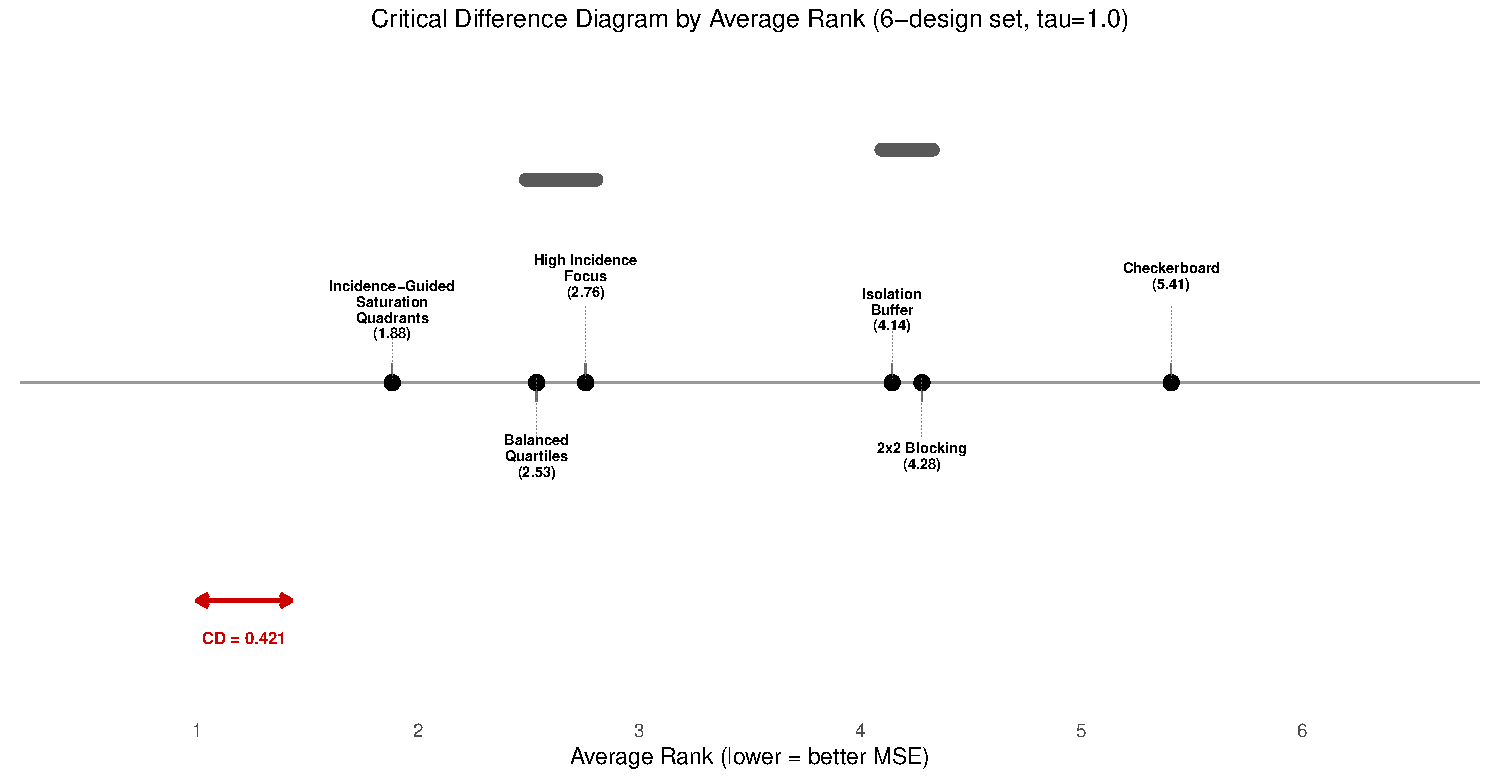
\includegraphics[width=0.85\linewidth]{figures/si_figures/si_fig_cd_diagram_rank.pdf}
\caption{Critical difference diagram by average Friedman rank (six retained
designs, $\tau=1.0$, all incidence configurations pooled). Designs are
positioned by average rank (lower = better MSE); the red arrow marks the
Nemenyi critical difference (CD = 0.421, $\alpha=0.05$). A bold bar connects
designs whose average ranks do not differ significantly.}
\label{fig:si-cd-rank}
\end{figure}

\begin{figure}[h]
\centering
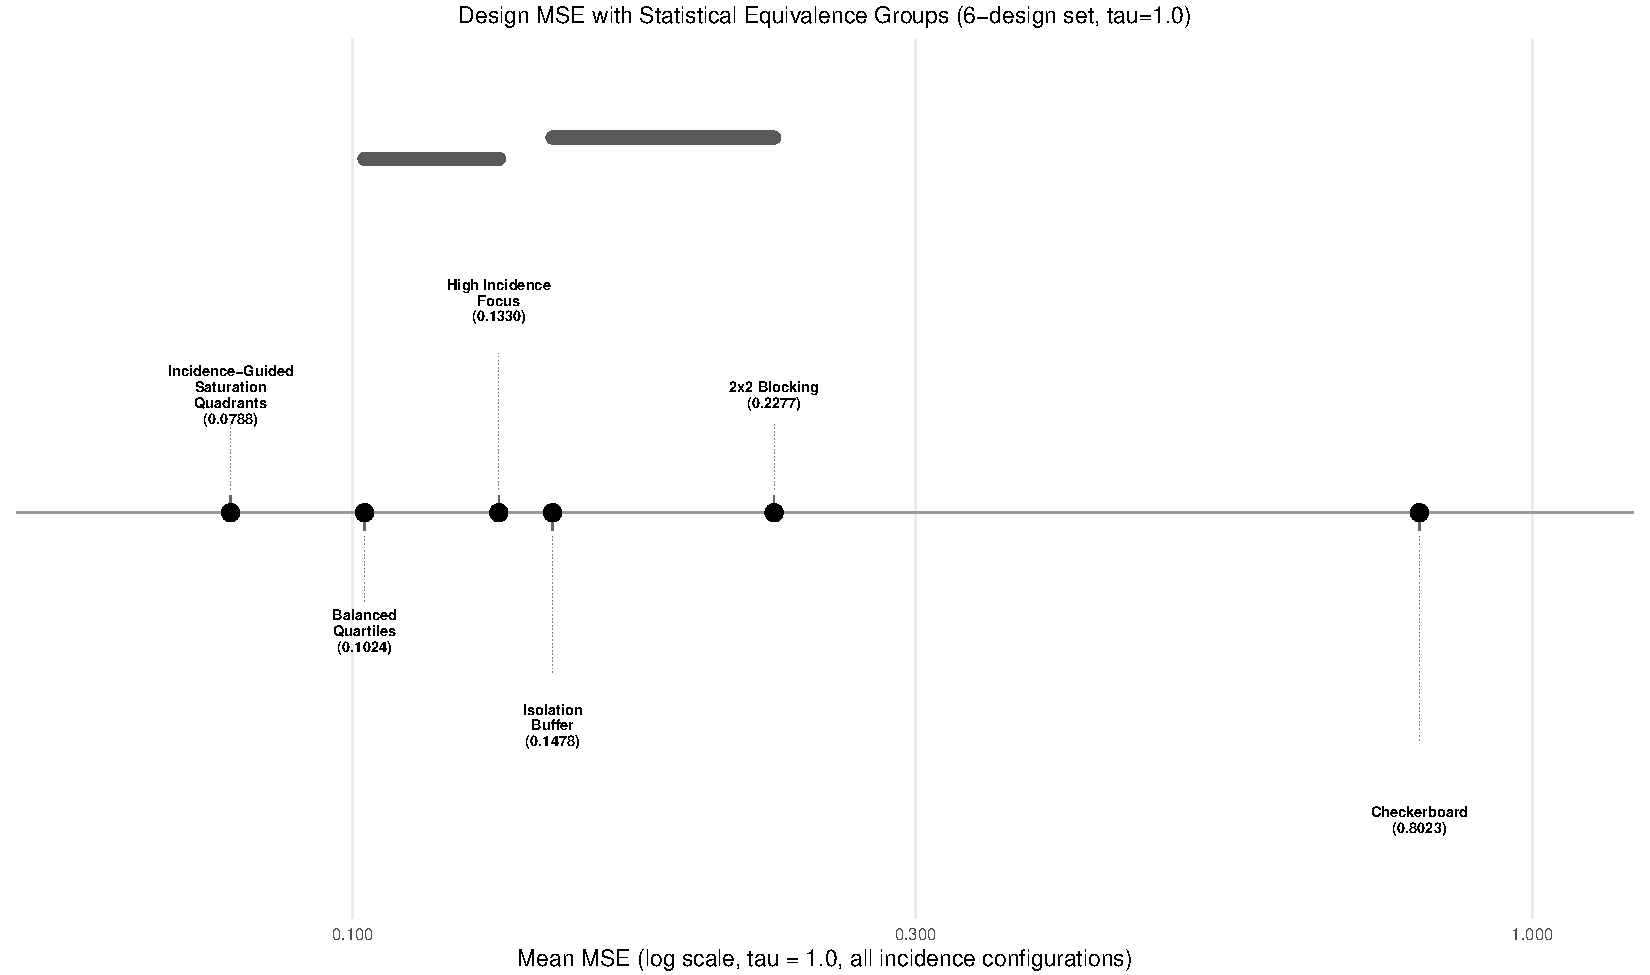
\includegraphics[width=0.85\linewidth]{figures/si_figures/si_fig_cd_diagram_mse.pdf}
\caption{The same six-design comparison as Figure~\ref{fig:si-cd-rank}, shown
by mean MSE on a log scale rather than average rank, to convey the practical
magnitude of the differences alongside their statistical grouping.}
\label{fig:si-cd-mse}
\end{figure}

\begin{table}[h]
\centering
\small
\caption{Mean MSE by design within each incidence-generating configuration
($\tau=1.0$, six retained designs). Designs are listed in the pooled best-to-worst
order from Table~2 of the main text; the best design within each column is
bolded.}
\begin{tabular}{lccccc}
\toprule
Design & \shortstack{iid\\Uniform} & \shortstack{Poisson\\$\rho_X{=}0.20$} & \shortstack{Poisson\\$\rho_X{=}0.50$} & \shortstack{Spatial\\$\rho_X{=}0.20$} & \shortstack{Spatial\\$\rho_X{=}0.50$} \\
\midrule
Incidence-Guided Sat.\ Quad. & \textbf{0.0800} & \textbf{0.0778} & \textbf{0.0811} & \textbf{0.0778} & \textbf{0.0774} \\
Balanced Quartiles           & 0.1000 & 0.1076 & 0.1024 & 0.1007 & 0.1012 \\
High Incidence Focus         & \textbf{0.0800} & 0.2017 & 0.2072 & 0.0982 & 0.0781 \\
Isolation Buffer             & 0.1468 & 0.1472 & 0.1447 & 0.1504 & 0.1498 \\
2$\times$2 Blocking          & 0.2258 & 0.2315 & 0.2300 & 0.2291 & 0.2221 \\
Checkerboard                 & 1.0586 & 0.9211 & 0.6944 & 0.7911 & 0.5461 \\
\bottomrule
\end{tabular}
\end{table}

Incidence-Guided Saturation Quadrants is the best or statistically tied-for-best
design in every incidence configuration tested. High Incidence Focus is
essentially tied with it under iid Uniform incidence (0.0800 vs.\ 0.0800, since
an uninformative incidence surface makes ``top half by incidence'' close to a
random half-split) but degrades sharply under Poisson incidence (MSE roughly
2.5$\times$ higher than its best-case values), because Poisson incidence is
count-based and noisier at the per-cluster level, making the observed median
split a less reliable proxy for the underlying risk surface a trial team would
actually want to target. Checkerboard's absolute MSE varies substantially by
configuration (0.546 to 1.059) but remains far worse than every other design in
all five configurations.

\section{Parameter Sensitivity}
\label{sec:s8}

\begin{table}[h]
\centering
\caption{Mean MSE by design and outcome spatial dependence $\rho$ ($\tau=1.0$,
six retained designs, pooled over neighbor type, $\gamma$, and spillover
regime).}
\begin{tabular}{lcccc}
\toprule
Design & $\rho=0.00$ & $\rho=0.01$ & $\rho=0.20$ & $\rho=0.50$ \\
\midrule
Incidence-Guided Sat.\ Quad. & 0.0823 & 0.0769 & 0.0755 & 0.0807 \\
Balanced Quartiles           & 0.1003 & 0.1009 & 0.1014 & 0.1069 \\
High Incidence Focus         & 0.1097 & 0.1180 & 0.1476 & 0.1570 \\
Isolation Buffer             & 0.1480 & 0.1431 & 0.1501 & 0.1498 \\
2$\times$2 Blocking          & 0.2306 & 0.2219 & 0.2278 & 0.2304 \\
Checkerboard                 & 0.7146 & 0.7458 & 0.9922 & 0.7566 \\
\bottomrule
\end{tabular}
\end{table}

\begin{table}[h]
\centering
\caption{Mean MSE by design and spillover magnitude $\gamma$ ($\tau=1.0$, six
retained designs, pooled over neighbor type, $\rho$, and spillover regime).}
\begin{tabular}{lcccc}
\toprule
Design & $\gamma=0.5$ & $\gamma=0.6$ & $\gamma=0.7$ & $\gamma=0.8$ \\
\midrule
Incidence-Guided Sat.\ Quad. & 0.0794 & 0.0792 & 0.0781 & 0.0787 \\
Balanced Quartiles           & 0.1011 & 0.1030 & 0.1049 & 0.1005 \\
High Incidence Focus         & 0.1330 & 0.1330 & 0.1331 & 0.1331 \\
Isolation Buffer             & 0.1450 & 0.1477 & 0.1493 & 0.1490 \\
2$\times$2 Blocking          & 0.2314 & 0.2287 & 0.2229 & 0.2278 \\
Checkerboard                 & 0.7101 & 0.7648 & 0.8297 & 0.9046 \\
\bottomrule
\end{tabular}
\end{table}

\begin{table}[h]
\centering
\caption{Mean MSE by design and spillover exposure regime ($\tau=1.0$, six
retained designs, pooled over neighbor type, $\rho$, and $\gamma$).}
\begin{tabular}{lcc}
\toprule
Design & Both & Control only \\
\midrule
Incidence-Guided Sat.\ Quad. & 0.0445 & 0.1132 \\
Balanced Quartiles           & 0.0435 & 0.1612 \\
High Incidence Focus         & 0.1043 & 0.1618 \\
Isolation Buffer             & 0.1479 & 0.1476 \\
2$\times$2 Blocking          & 0.0575 & 0.3979 \\
Checkerboard                 & 0.2816 & 1.3230 \\
\bottomrule
\end{tabular}
\end{table}

Figures~\ref{fig:si-mse-heatmap} and \ref{fig:si-rank-heatmap} show the same
$\rho$-by-design pattern as a heatmap (Poisson $\rho_X=0.20$ representative
configuration, both neighbor types), confirming that absolute MSE rises with
$\rho$ for every design but the design ranking is unchanged at every $\rho$
level. Neither outcome spatial dependence ($\rho$) nor spillover magnitude
($\gamma$) meaningfully changes which design is best; both increase absolute
MSE for every design (most visibly for Checkerboard, whose MSE roughly doubles
from $\gamma=0.5$ to $\gamma=0.8$: 0.710 to 0.905). The spillover exposure
regime shows the largest relative effect: every design's MSE is 2--5$\times$
higher under \texttt{control\_only} spillover than under \texttt{both}, because
concentrating spillover exposure entirely on control clusters creates a sharper
asymmetry between treated and control outcomes than the direct treatment effect
alone; Checkerboard is affected most severely (0.282 to 1.323, a
4.7$\times$ increase) because its rigid spatial alternation maximizes the
number of control clusters adjacent to a treated cluster.

\begin{figure}[h]
\centering
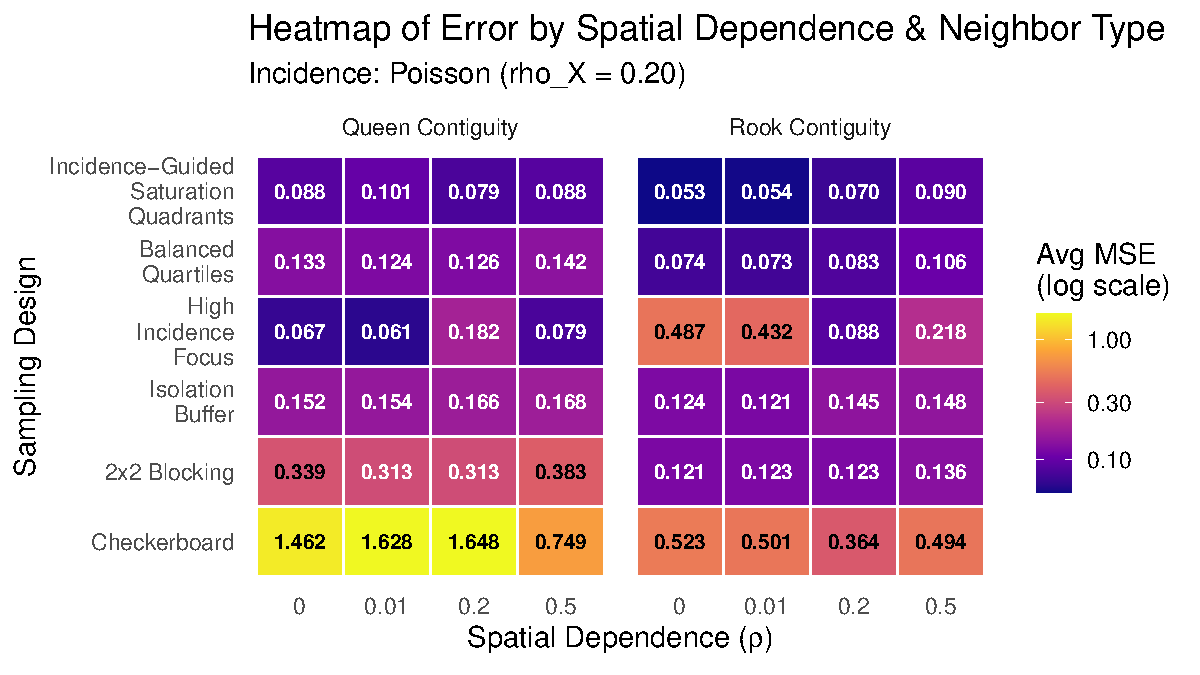
\includegraphics[width=0.85\linewidth]{figures/si_figures/si_fig_mse_heatmap.pdf}
\caption{Mean MSE by design and outcome spatial dependence $\rho$, Poisson
incidence ($\rho_X=0.20$, $\tau=1.0$), by neighbor type. Color scale is
log-transformed to distinguish designs in the low-MSE range. Rows are ordered
best (top) to worst (bottom) by pooled mean MSE.}
\label{fig:si-mse-heatmap}
\end{figure}

\begin{figure}[h]
\centering
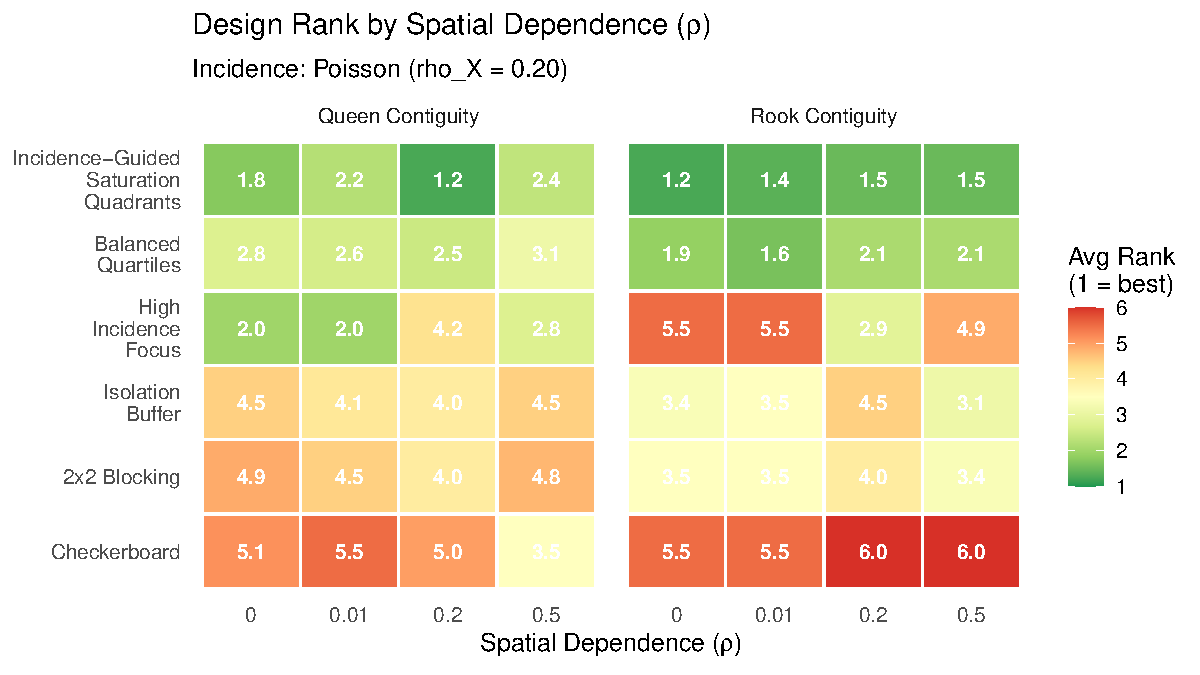
\includegraphics[width=0.85\linewidth]{figures/si_figures/si_fig_rank_heatmap.pdf}
\caption{Average Friedman rank by design and outcome spatial dependence $\rho$,
Poisson incidence ($\rho_X=0.20$, $\tau=1.0$), by neighbor type (rank 1 =
lowest MSE = best, averaged over $\gamma$ and spillover regime). Rows are
ordered best (top) to worst (bottom).}
\label{fig:si-rank-heatmap}
\end{figure}

\begin{figure}[h]
\centering
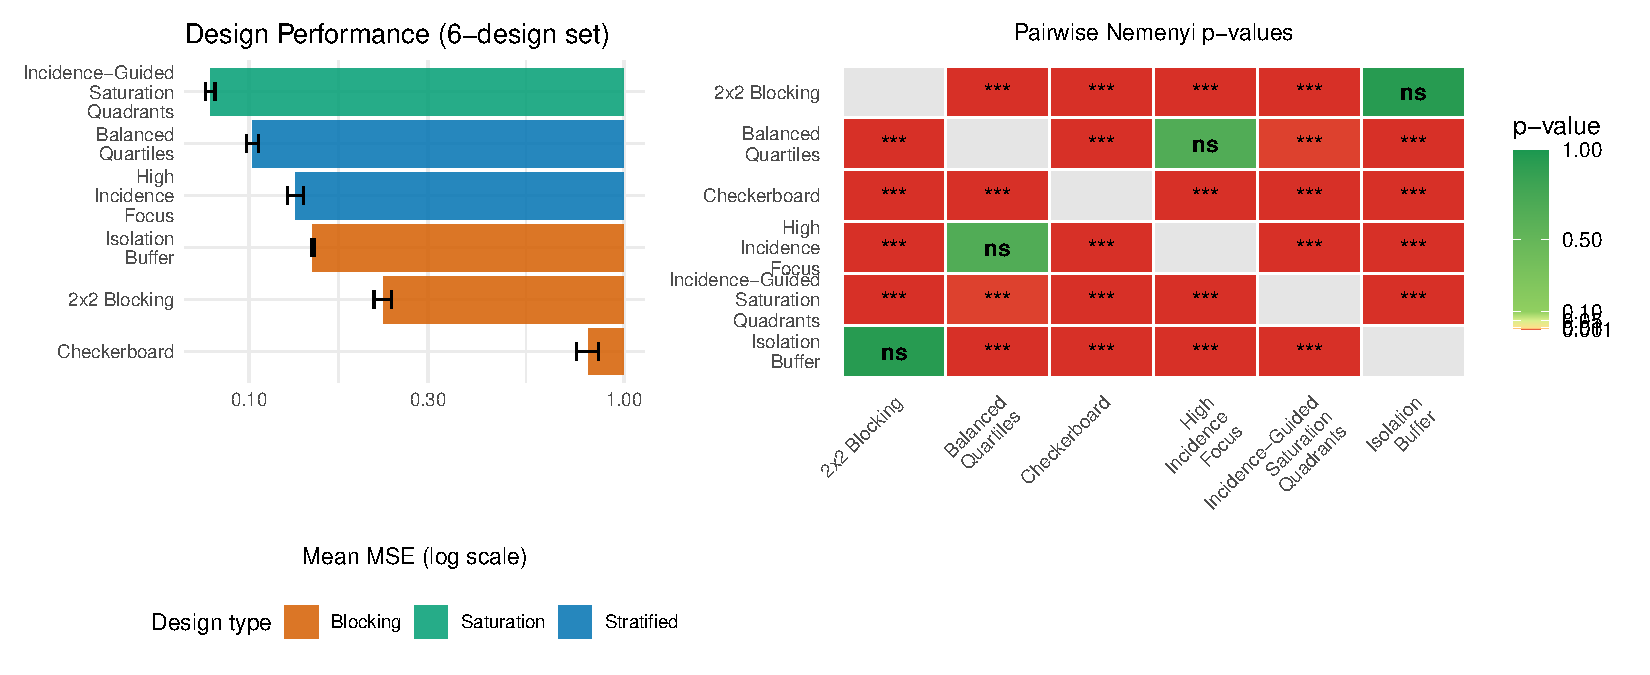
\includegraphics[width=\linewidth]{figures/si_figures/si_fig_performance_pvalue_twopanel.pdf}
\caption{Left: mean MSE per design (log scale, $\tau=1.0$) with $\pm1$ standard
error bars, colored by conceptual design group (Blocking: Checkerboard,
2$\times$2 Blocking, Isolation Buffer; Stratified: High Incidence Focus,
Balanced Quartiles; Saturation: Incidence-Guided Saturation Quadrants). Right:
pairwise Nemenyi $p$-value heatmap for the six retained designs; dark red cells
are statistically significant ($p<0.05$).}
\label{fig:si-twopanel}
\end{figure}

\section{Effect-Size (Tau) Sensitivity and Rank Stability}
\label{sec:s9}

\begin{table}[h]
\centering
\caption{Friedman omnibus test for design differences, stratified by true
treatment effect $\tau$ (six retained designs, 320 blocks per stratum). All
strata reject the null of equal design ranks.}
\begin{tabular}{lccc}
\toprule
$\tau$ & $\chi^2$ (df$=5$) & $p$-value & $N$ blocks \\
\midrule
0.8 & 730.60 & $<2\times10^{-16}$ & 320 \\
1.0 & 800.88 & $<2\times10^{-16}$ & 320 \\
1.5 & 705.71 & $<2\times10^{-16}$ & 320 \\
2.0 & 658.46 & $<2\times10^{-16}$ & 320 \\
3.0 & 557.29 & $<2\times10^{-16}$ & 320 \\
\bottomrule
\end{tabular}
\end{table}

The Friedman statistic declines monotonically as $\tau$ increases (from 730.6
at $\tau=0.8$ to 557.3 at $\tau=3.0$), consistent with a compression of relative
design differences at larger true effect sizes: a larger direct effect is
easier for every design to estimate, narrowing the MSE gap between the best and
worst designs even though the ordering itself does not change (main text
Results; Figure~\ref{fig:si-tau-mse}). Despite this compression, every stratum
remains overwhelmingly significant, and Incidence-Guided Saturation Quadrants
and Balanced Quartiles remain the top two designs at every tested $\tau$
(Figure~\ref{fig:si-tau-mse}), while Checkerboard's coverage remains severely
sub-nominal across the full $\tau$ range (Figure~\ref{fig:si-tau-coverage}),
confirming that its inferential failure is a design property, not an artifact
of the specific effect size used in the primary comparison.

\begin{figure}[h]
\centering
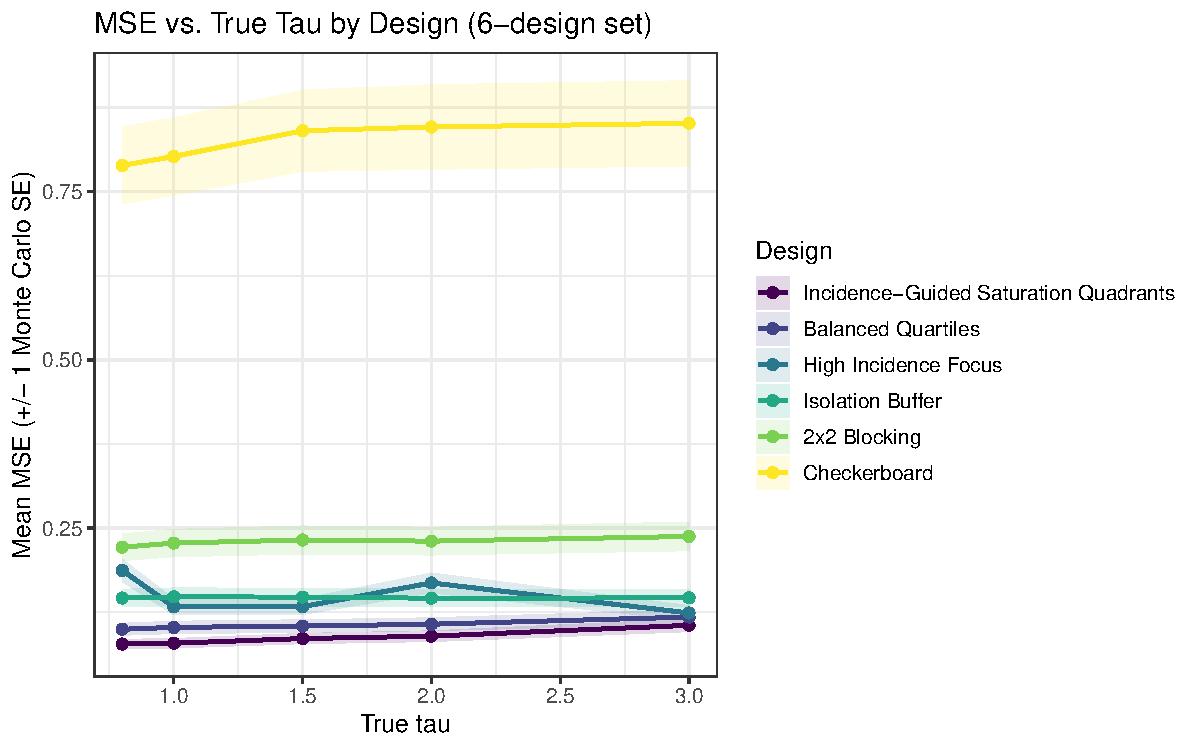
\includegraphics[width=0.85\linewidth]{figures/si_figures/si_fig_tau_mse.pdf}
\caption{Mean MSE by design across the five tested treatment-effect magnitudes
($\tau\in\{0.8,1.0,1.5,2.0,3.0\}$), with $\pm1$ Monte Carlo standard error
ribbons. Legend is ordered best to worst by pooled $\tau=1.0$ MSE.}
\label{fig:si-tau-mse}
\end{figure}

\begin{figure}[h]
\centering
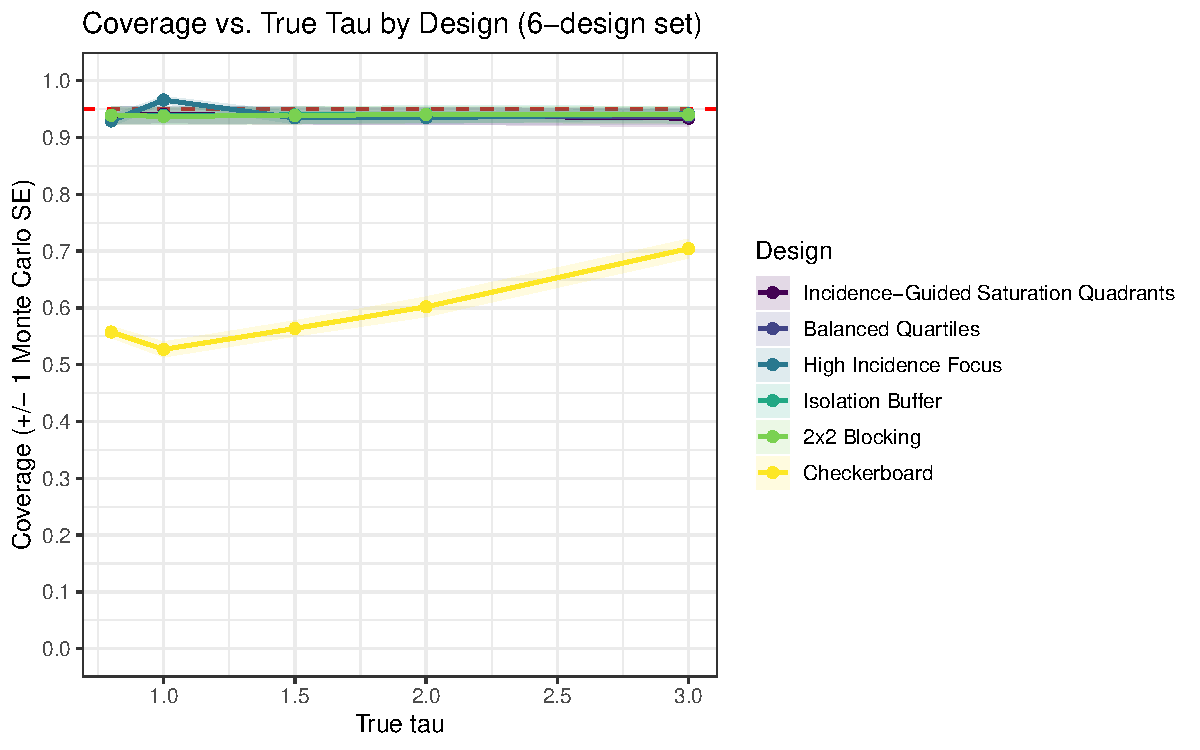
\includegraphics[width=0.85\linewidth]{figures/si_figures/si_fig_tau_coverage.pdf}
\caption{95\% confidence interval coverage by design across the five tested
treatment-effect magnitudes, with $\pm1$ Monte Carlo standard error ribbons.
The dashed red line marks the nominal 95\% level.}
\label{fig:si-tau-coverage}
\end{figure}

\section{Subgroup Robustness and Win Rate}
\label{sec:s10}

\begin{table}[h]
\centering
\caption{MSE quantiles across all 320 scenario blocks per design ($\tau=1.0$,
six retained designs), sorted by median MSE.}
\begin{tabular}{lccccc}
\toprule
Design & Best & Q25 & Median & Q75 & Worst \\
\midrule
Incidence-Guided Sat.\ Quad. & 0.0344 & 0.0441 & 0.0591 & 0.1085 & 0.1894 \\
Balanced Quartiles           & 0.0332 & 0.0432 & 0.0764 & 0.1664 & 0.2743 \\
High Incidence Focus         & 0.0125 & 0.0510 & 0.0855 & 0.1658 & 0.5039 \\
2$\times$2 Blocking          & 0.0395 & 0.0572 & 0.1201 & 0.3111 & 0.8210 \\
Isolation Buffer             & 0.1018 & 0.1312 & 0.1464 & 0.1637 & 0.2057 \\
Checkerboard                 & 0.0331 & 0.1904 & 0.4556 & 0.8167 & 4.8117 \\
\bottomrule
\end{tabular}
\end{table}

Table order above follows median MSE (the ordering used elsewhere for the
robustness profile), which differs slightly from the pooled-mean-MSE ordering
used in the main text: Isolation Buffer has a higher median MSE than
2$\times$2 Blocking but a much narrower spread (worst-case 0.206 vs.\ 0.821),
making it the more consistent of the two even though its typical-case MSE is
worse. Checkerboard's best-case MSE (0.033, achieved only under the most
favorable spatial/spillover configuration) is competitive with the top
designs, but its worst-case MSE (4.81) is roughly an order of magnitude
larger than any other design's worst case, illustrating that its poor pooled
average reflects catastrophic failure in a subset of configurations rather
than uniformly mediocre performance.

\begin{table}[h]
\centering
\caption{Win rate: fraction of the 320 scenario blocks ($\tau=1.0$) in which
each design achieves the lowest MSE among the six retained designs.}
\begin{tabular}{lc}
\toprule
Design & Win rate \\
\midrule
High Incidence Focus                  & 0.3656 \\
Incidence-Guided Saturation Quadrants & 0.3594 \\
Balanced Quartiles                    & 0.1906 \\
Checkerboard                          & 0.0500 \\
Isolation Buffer                      & 0.0250 \\
2$\times$2 Blocking                   & 0.0094 \\
\bottomrule
\end{tabular}
\end{table}

High Incidence Focus and Incidence-Guided Saturation Quadrants together win
72.5\% of all scenario blocks, consistent with Section~\ref{sec:s7}'s finding
that High Incidence Focus is highly competitive under favorable
(low-noise/informative) incidence configurations even though its pooled-average
MSE is substantially worse than Incidence-Guided Saturation Quadrants once
Poisson-incidence configurations are included. Checkerboard's 5\% win rate
confirms it is occasionally competitive (its best-case MSE in the table above)
but is the wrong default choice for the large majority of realistic spatial and
spillover conditions.

\section{Application-Scale Illustration: Six-Design Subset}
\label{sec:s11}

\textbf{As in the main text, these numbers use a synthetic, placeholder
incidence surface and must not be interpreted as a design recommendation for
the real SUD application}; they will be superseded once the real
SUDDEN-derived North Carolina county dataset is finalized.

\begin{table}[h]
\centering
\caption{Mean MSE, coverage, and power for the six retained designs on the
58-cluster North Carolina community-college application geography ($\tau=1.0$,
averaged over $\gamma$, $\rho$, and spillover regime). Design names are the
application study's own labels (\texttt{application\_designs.R}); see note
below for two relabelings relative to the primary grid-based study.}
\begin{tabular}{lccc}
\toprule
Design (application label) & MSE & Coverage & Power \\
\midrule
Balanced Quartiles                    & 0.0701 & 0.938 & 0.971 \\
Incidence-Guided Saturation Regions   & 0.0778 & 0.934 & 0.966 \\
2$\times$2 Blocking                   & 0.0782 & 0.928 & 0.961 \\
Block Stratified Sampling             & 0.2323 & 0.930 & 0.592 \\
Isolation Buffer                      & 0.2649 & 0.938 & 0.553 \\
High Incidence Focus                  & 0.2686 & 0.939 & 0.535 \\
\bottomrule
\end{tabular}
\end{table}

\textit{Note on design relabeling.} The application study renames two designs
for the irregular, real-world community-college geography, where the grid
study's terms do not apply literally. Design ID 1 (Checkerboard on the regular
$10\times10$ grid) is implemented as \textbf{Block Stratified Sampling} on the
irregular map --- a block-stratified analog of the alternating-grid concept,
since a literal checkerboard pattern has no meaning without regular grid cells.
Design ID 8 (Incidence-Guided Saturation Quadrants on the grid) is implemented
as \textbf{Incidence-Guided Saturation Regions}, replacing the four literal
2$\times$2 grid quadrants with four population-balanced $k$-means regions,
since quadrants likewise have no meaning on an irregular map. Both are the
application study's own design names, used verbatim in the table above rather
than translated back to the grid-study terminology, to avoid implying the
application implementation is identical to the grid-study mechanism.

The qualitative pattern is broadly consistent with the primary grid-based
results: incidence-stratified and saturation-based designs (Balanced
Quartiles, Incidence-Guided Saturation Regions, 2$\times$2 Blocking) achieve
the lowest MSE and highest power, while Block Stratified Sampling, Isolation
Buffer, and High Incidence Focus are clearly worse on both dimensions. Two
notable differences from the grid study: 2$\times$2 Blocking, which performed
poorly (rank 5 of 6) on the regular grid, is competitive here (rank 3),
plausibly because its application-scale implementation uses local spatial
blocks defined from cluster centroids, incidence, and population rather than
literal $2\times2$ grid cells; and High Incidence Focus, which was competitive
on the grid, is one of the three worst designs here, consistent with its
grid-study sensitivity to how informative the observed incidence surface is
(Section~\ref{sec:s7}) --- the NC community-college incidence surface used for
this placeholder illustration may be less informative for top-half targeting
than the grid study's iid or spatial configurations. All coverage values
remain near the nominal 95\% level except for Block Stratified Sampling
(93.0\%), which nonetheless does not show the severe under-coverage seen for
Checkerboard on the regular grid (52.7\%) --- a difference attributable to the
irregular map's block-stratified adaptation not reproducing the same
worst-case $Z$/$WZ$ collinearity as the literal alternating grid pattern.

\end{document}
